\ifx allfiles undefined
\documentclass[a4paper,10pt]{article}
\usepackage{CJK}
\usepackage{indentfirst}
\usepackage{graphicx}

%%%代码
\usepackage{color}
\usepackage{xcolor}
\definecolor{keywordcolor}{rgb}{0.8,0.1,0.5}
\usepackage{listings}
\lstset{breaklines}%这条命令可以让LaTeX自动将长的代码行换行排版
\lstset{extendedchars=false}%这一条命令可以解决代码跨页时,章节标题,页眉等汉字不显示的问题
\lstset{language=C++, %用于设置语言为C++
    keywordstyle=\color{keywordcolor} \bfseries, %设置关键词
    identifierstyle=,
    basicstyle=\ttfamily, 
    commentstyle=\color{blue} \textit,
    stringstyle=\ttfamily, 
    showstringspaces=false,
    %frame=shadowbox, %边框
    captionpos=b
}
%%%

%\hypersetup{CJKbookmarks=true} %解决section不能使用中文的问题

\begin{document}
\begin{CJK}{UTF8}{gbsn}     %CJK:支持中文

\else

动态规划是运筹学的一个分支,是求解决策过程(decision process)最优化的数学方法,它将多阶段过程转换为一系列多阶段问题,利用各个阶段之间的关系逐个求解.动态规划的方法的基础是最优子结构和子问题重叠,无后效性.\\
\\
最优子结构意味着当前问题的最优解包含了子问题的最优解.在论证问题的最优子结构性质时可以使用"cut-and-paste"的方法,即假设子问题的解并非最优解,然后"cut"非最优子问题,"paste"最优解来导出出矛盾.\\
\\
子问题独立(无后效性)意味着将某个问题划分为多个stage时,各个stage并不使用共同的资源(矩阵连乘中子矩阵相互独立[并行的],最短路径中先后选取的两条路径无多于一个公共节点[先后的]).对于子阶段并不相互独立的情况(最长路径中两条路径可能使用公共节点),不能使用动态规划来求解.\\
\\
子问题重叠意味着求解问题时,可能需要反复的求解某些子问题,动态规划方法中通过使用备忘录来记录已求解的子问题来避免重复的计算,可以常数时间内查看.[注意,适合分治法来处理的问题的子问题都是互异的.]\\
\\
动态规划以自底向上的方法来进行阶段(stage)决策(decision),首先获取某阶段(stage)的最优解,以此来计算后一阶段(stage).具体的实现可以分为两种:(1)Top-down,Recursive.这种方法的好处是能自动的处理计算顺序,子问题总是被先计算;只会处理必要的自问题,不需要处理全部的状态空间.缺点是采用递归的结构,执行效率差;无法自由的控制计算顺序,导致无法妥善使用存储空间;(2)Bottom-up,Iterative.大体来讲,动态规划方法的复杂度依赖于子阶段(state)的总个数和每个子问题的状态(state)的乘积.\\
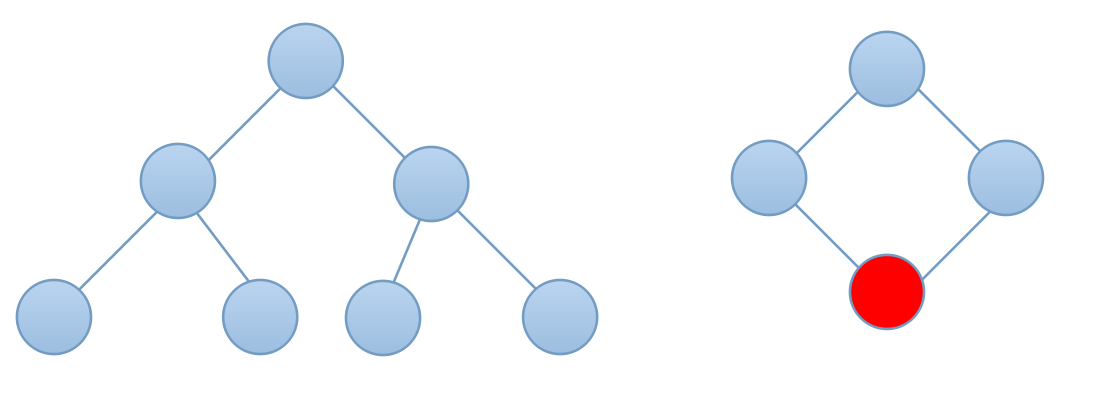
\includegraphics[width=0.5\textwidth]{Dynamic-Programming/background/pics0}
\\
注意:描述子问题的空间时,可以遵循从简到繁的步骤.尽量使用最简单的空间来解决问题(维度最小).\\
\\

\fi

\ifx allfiles undefined
\end{CJK}
\end{document}
\fi
